\subsection{Simulated Rapid Tests}
\label{subsec:results_rapid_test_statistics}

In order to make most use out of limited data sources on rapid test usage, we model the
number of performed rapid tests as a result of time invariant willingness to do rapid
tests and time varying supply side factors and events that trigger rapid tests. Thus, the
$\pi$ parameters governing when individuals do rapid tests described in
Section~\ref{subsec:rapid_test_demand} are only indirectly related to the number of rapid
tests that are actually performed in the model. When it comes to positive and negative
rapid tests, there is even an additional layer because rapid tests are imperfectly
sensitive and specific.

In this section we look at how rapid tests expanded in our simulations over time and to
what degree they are useful as a screening device despite their imperfections.

We start with the share of the population doing a rapid test, receiving a positive rapid
test and receiving a negative rapid test over time by the channel through which the test
was demanded in Figures~\ref{fig:rapid_test_demand_by_channel},
\ref{fig:pos_rapid_tests_by_channel} and \ref{fig:neg_rapid_tests_by_channel},
respectively. Overall, the share of the population getting a rapid test on a given day
increases from 2\% in mid March to over 10\% by May. The work rapid tests are a little
ragged because of public holidays. For education rapid tests both vacations (first half
of April) as well as the opening of schools in May are very visible in the rapid test
demand. Overall, work tests make up the largest fraction of rapid tests. The image is
very similar for the share of positive tests, except that the overall number of positive
tests starts decreasing in May as rapid test expansion comes to a halt and cases fall,
especially the positive share of private rapid tests falls as less and less individuals
are triggered to seek a rapid test because of a risk contact in their household.

\begin{figure}[ht] % Share tested per day
    \centering
    \begin{subfigure}[b]{0.49\textwidth}
        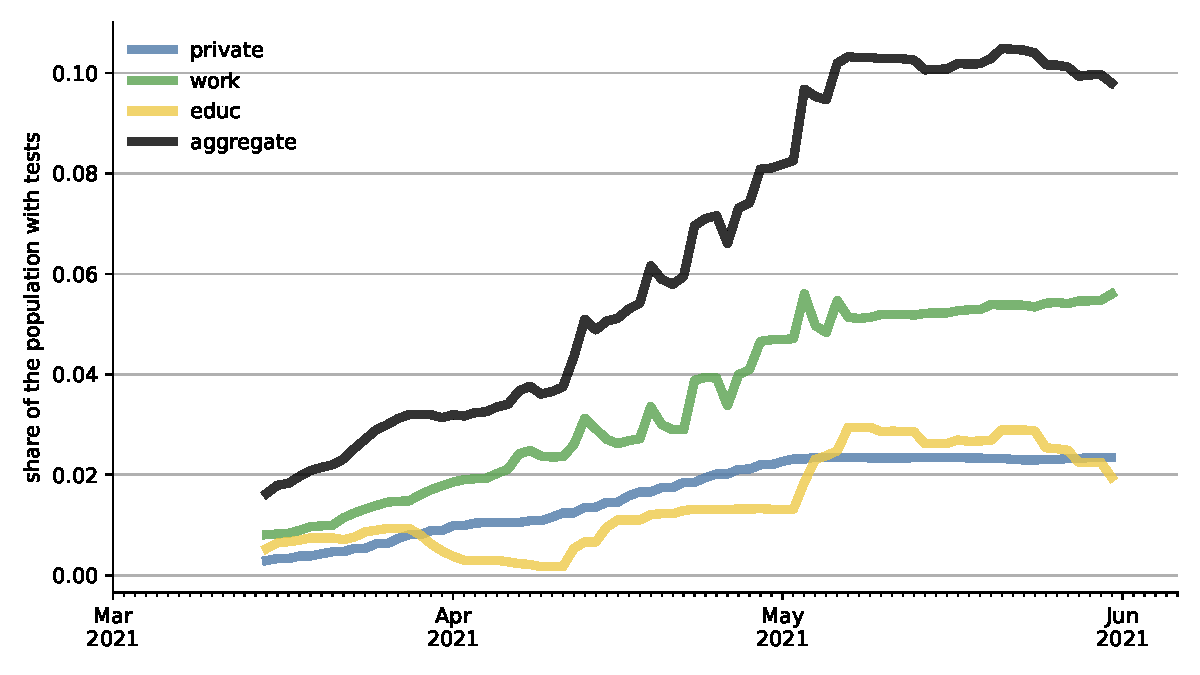
\includegraphics[width=\textwidth]{figures/results/figures/rapid_test_statistics/popshare_tested}
        \caption{Share of the Population Doing a Rapid Test on a Given Day, by Channels}
        \label{fig:rapid_test_demand_by_channel}
    \end{subfigure}
    \hfill
    \begin{subfigure}[b]{0.49\textwidth}
        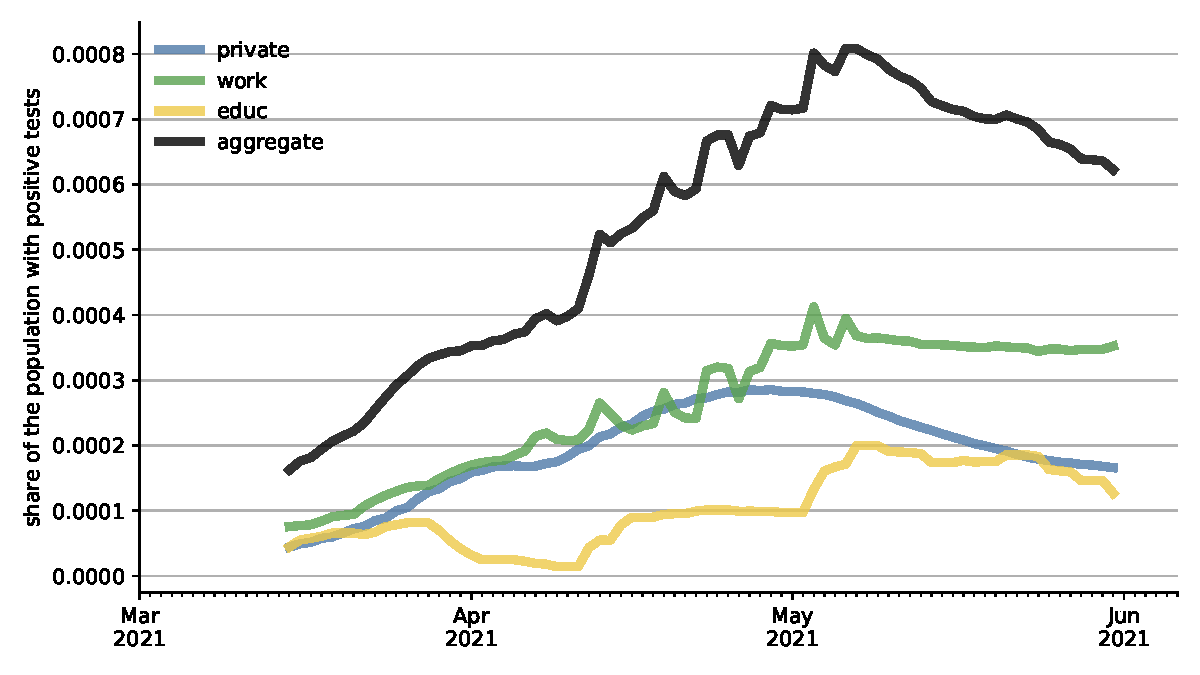
\includegraphics[width=\textwidth]{figures/results/figures/rapid_test_statistics/popshare_tested_positive}
        \caption{Share of the Population Testing Positive on a Given Day, by Channels}
        \label{fig:pos_rapid_tests_by_channel}
    \end{subfigure}
    \caption{Rapid Test Shares in the Population by Channel}
    \floatfoot{\noindent \textit{Note:}
        Rapid tests in the education setting are demanded by teachers (nursery,
        preschool and school) as well as pupils. After Easter the required frequency of
        tests is increased from once per week to twice per week. Work rapid tests are
        demanded by individuals that still have work contacts, i.e. do not work from
        home. The share of employers offering rapid tests increases over the time frame
        and the frequency of testing is also increased. Private tests are demanded by
        individuals for one of three reasons: having developed symptoms without access
        to a PCR test, having a household member that has tested positive or developed
        symptoms or having planned a weekly meeting with friends.
        Panel~\subref{fig:rapid_test_demand_by_channel} shows the share of the
        population doing a rapid test on a given day.
        Panel~\subref{fig:pos_rapid_tests_by_channel} shows the share of the population
        testing positive on a given day (true and false positives).}
\end{figure}

\FloatBarrier

Next, we show the tests split by whether they are true positive, false positive, true
negative or false negative (see Figure~\ref{fig:rapid_test_results_numbers}) in numbers
per million individuals to make the metric comparable to incidences.
% true positive
The number of true positives (Figure~\ref{fig:rapid_tests_number_true_positive}) rapidly
increases and peaks at the end of April with over 200 cases per million detected through
rapid tests per day. This means that our model suggests that Germany was able to detect
up to 16,600 cases per day that would have likely gone undetected otherwise. The most
powerful tool for detecting cases are the private rapid tests. This is because a large
share of them are targeted, i.e. triggered by events in the household. However, this
does not mean that rapid tests in the workplace or at school are useless. It is rather
the combination of large scale screening at work and in schools and very efficient
follow up tests whenever those screening tests detected a case. Shapley values
(Figure~\ref{fig:2021_scenarios_decomposition_tests}) take this into account and
assign about 50\% of the overall reduction of case numbers via rapid tests to private
rapid tests with work and school rapid tests accounting for 40\% and 7\%,
respectively.

Such a large effect of rapid tests seems to be at odds with the general perception that
they are not very reliable. However, this is not the case,\comment[id=HM]{I do not
understand. 80 fals neg for 200 true pos does not seem too reliable? I guess the
important bit is the reference cat. -- catching 200 pos vs. nothing} which can be seen
from the number of false negative tests. At its peak at the beginning of May, there are
more than 80 false negative rapid tests per million inhabitants per day. While this
number might sound low in isolation, it becomes quite large when set in context: We
estimate that at at the the same time only 200 cases per million are detected by rapid
tests. This means that even at the time where discovery of cases via rapid tests is at
its peak, almost 30\% of people who are infected and make a test are not discovered by
the test.

This shows clearly that the large effect of rapid tests on the infection dynamic
is not driven by unrealistic assumptions about their sensitivity but rather by the
fact that there was a very large number of infected individuals who did not know they
are positive. Detecting and isolating some of them is enough to slow down the
overall infection dynamic.

\begin{figure}   % Number of True Positive / False Positive / True Negative / False Negative
    \centering
    \begin{subfigure}[b]{0.425\textwidth}
        \centering
        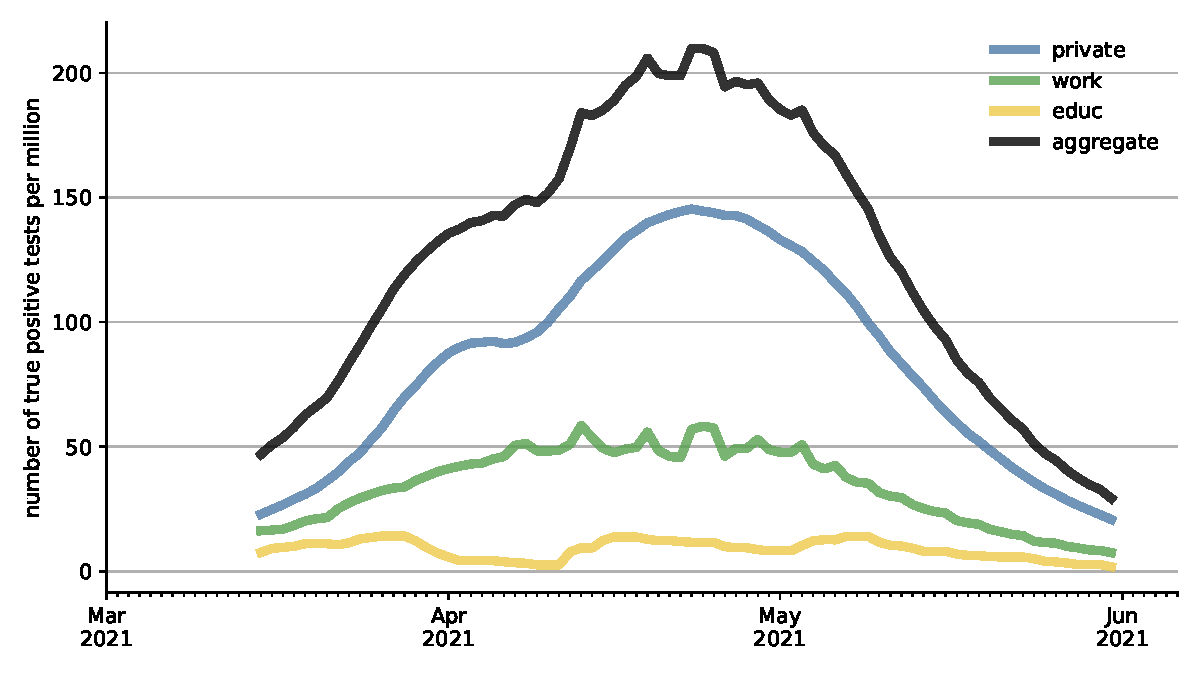
\includegraphics[width=\textwidth]{figures/results/figures/rapid_test_statistics/number_true_positive}
        \caption{Number of Discovered Cases Due to Rapid Tests by Channel}
        \label{fig:rapid_tests_number_true_positive}
    \end{subfigure}
    \hfill
    \begin{subfigure}[b]{0.425\textwidth}
        \centering
        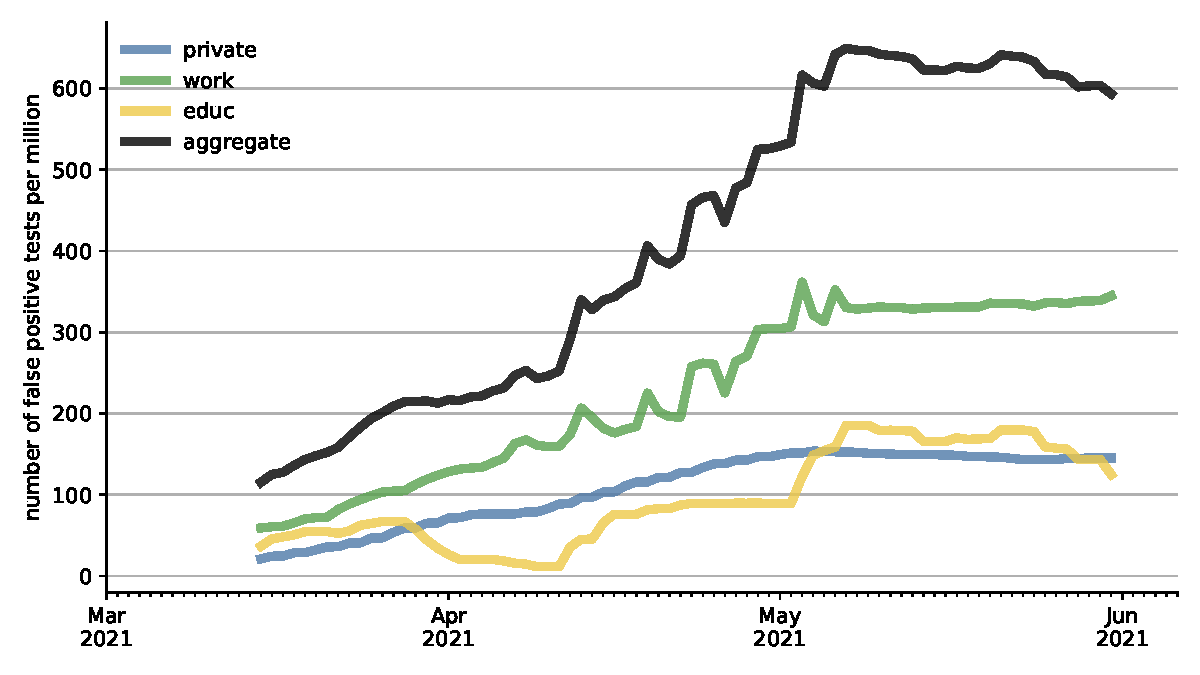
\includegraphics[width=\textwidth]{figures/results/figures/rapid_test_statistics/number_false_positive}
        \caption{Number of False Positive Rapid Tests by Channel}
        \label{fig:rapid_tests_number_false_positive}
    \end{subfigure}
    \vskip3ex
    \begin{subfigure}[b]{0.425\textwidth}
        \centering
        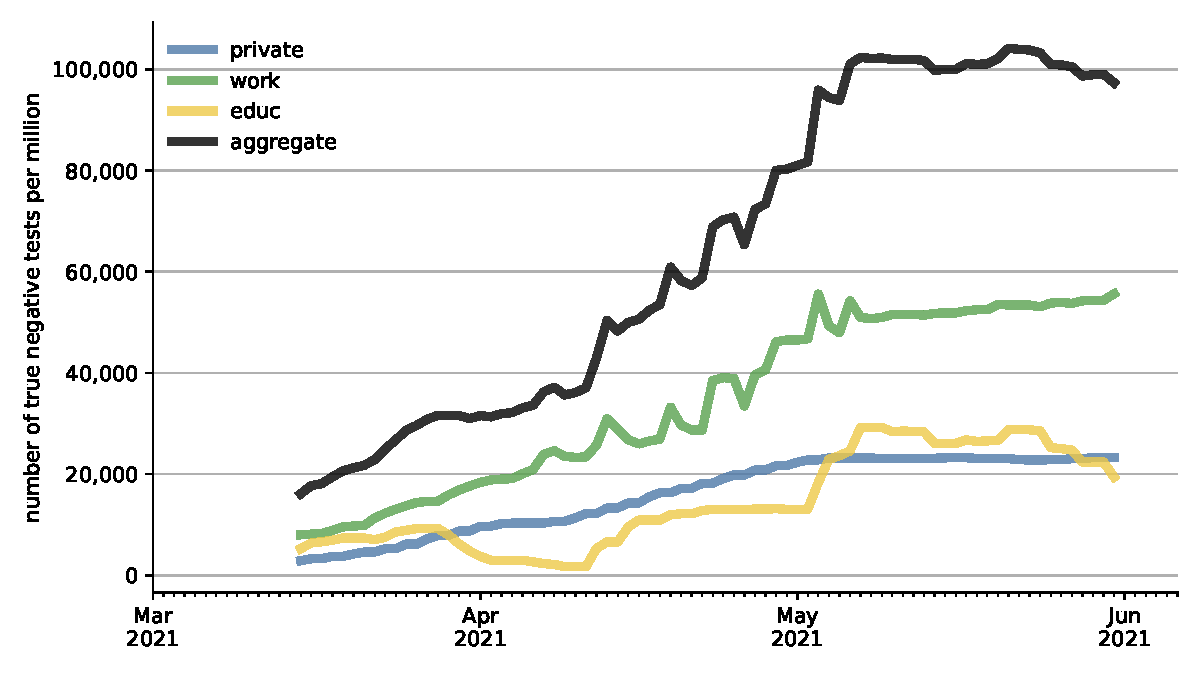
\includegraphics[width=\textwidth]{figures/results/figures/rapid_test_statistics/number_true_negative}
        \caption{Number of True Negative Rapid Tests by Channel}
        \label{fig:rapid_tests_number_true_negative}
    \end{subfigure}
    \hfill
    \begin{subfigure}[b]{0.425\textwidth}
        \centering
        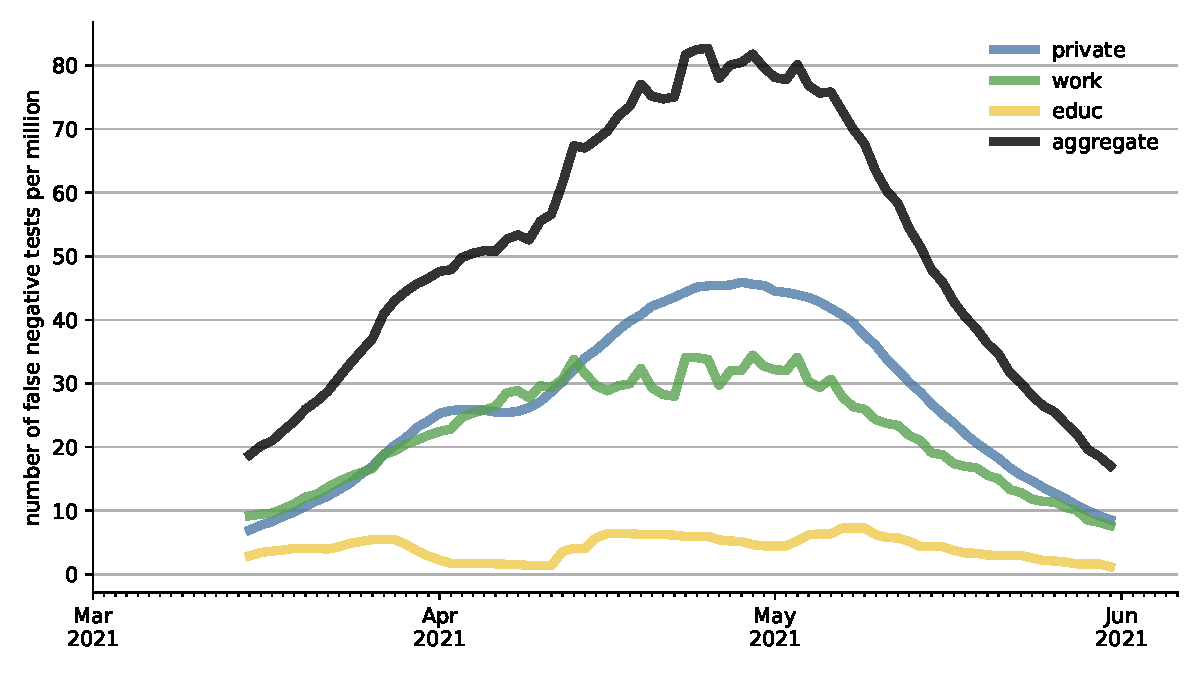
\includegraphics[width=\textwidth]{figures/results/figures/rapid_test_statistics/number_false_negative}
        \caption{Number of False Negative Rapid Tests by Channel}
        \label{fig:rapid_tests_number_false_negative}
    \end{subfigure}
    \vskip3ex
    \caption{Rapid Test Results}
    \label{fig:rapid_test_results_numbers}
    \floatfoot{\noindent \textit{Note:}
        Each panel shows the number of rapid tests per million inhabitants that fall into the
        respective category. Private rapid tests are especially good at detecting cases but
        since they are often triggered by rapid tests from other channels, the other groups
        of tests, especially rapid tests at the workplace, also play an important role for
        containing the pandemic.}
\end{figure}

\FloatBarrier

A similar picture arises, when looking at the false positive rate,
i.e. the share of positive tests that go to people who are not infected.
Figure~\ref{fig:rapid_tests_false_positive_rate} shows that the false
positive rate is very high. On average 60\% to 93\% of positive tests are
received by individuals that are not infected. The false positive rate increases over
time. This is due to the low prevalence of infections in the population, which falls
over time. Again, private rapid tests are an exception with a much lower false
positive rate because those tests are primarily demanded when there is a high likelihood
of being infected. The low false negative rate of 0.2\% looks very low. As discussed
above this is deceiving and just a mechanical consequence of a very low prevalence
of the disease and the many rapid tests done by non-infected people.

\begin{figure} % True Positive / False Positive / True Negative / False Negative Rate
    \centering
    % \begin{subfigure}[b]{0.425\textwidth}
    %     \centering
    %     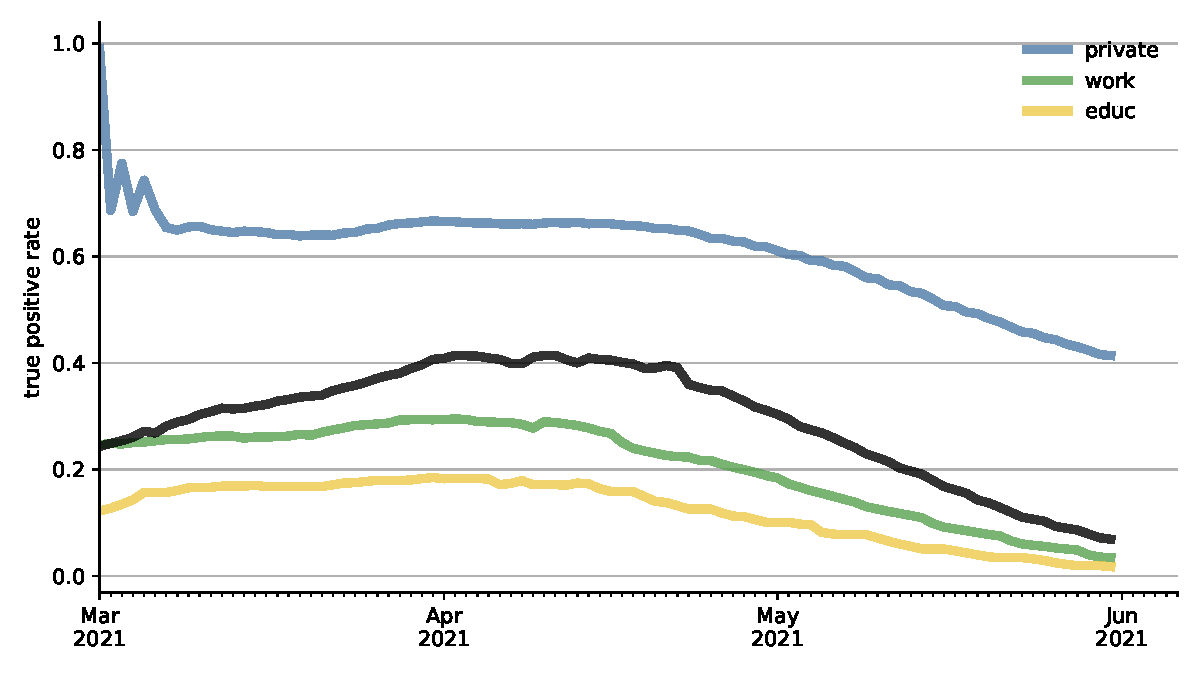
\includegraphics[width=\textwidth]{figures/results/figures/rapid_test_statistics/true_positive_rate}
    %     \caption{Rate of True Positive Rapid Tests by Channel}
    %     \label{fig:rapid_tests_true_positive_rate}
    % \end{subfigure}
    % \hfill
    \begin{subfigure}[b]{0.425\textwidth}
        \centering
        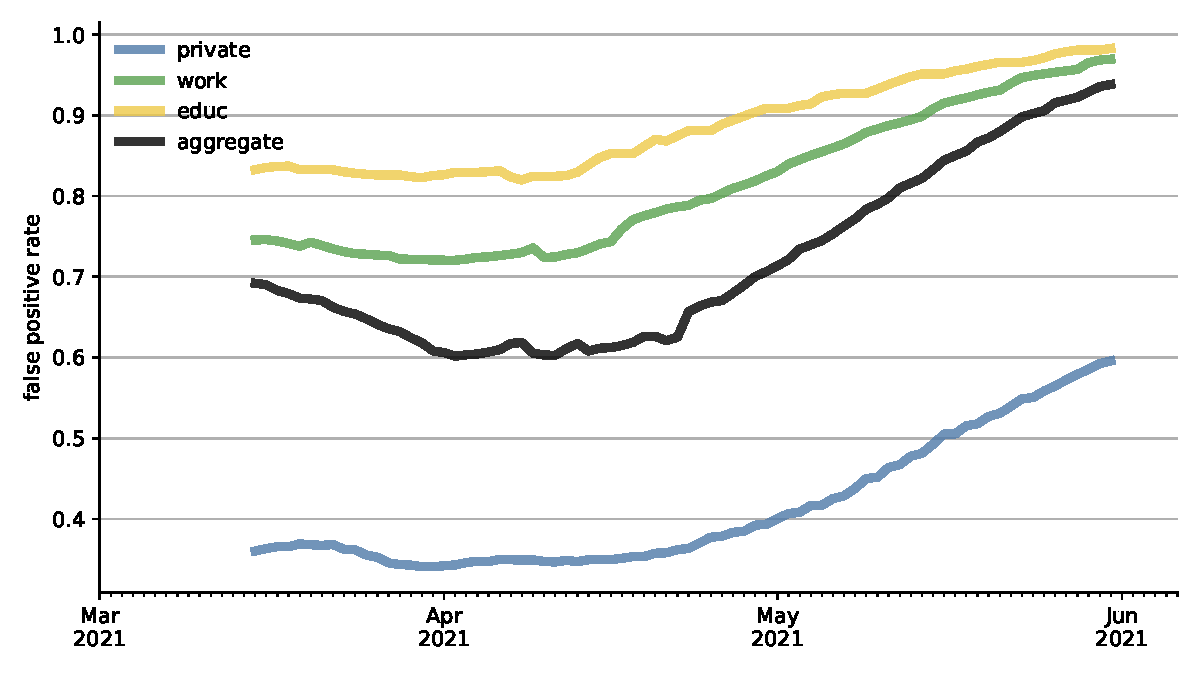
\includegraphics[width=\textwidth]{figures/results/figures/rapid_test_statistics/false_positive_rate}
        \caption{Rate of False Positive Rapid Tests by Channel}
        \label{fig:rapid_tests_false_positive_rate}
    \end{subfigure}
    % \vskip3ex
    % \begin{subfigure}[b]{0.425\textwidth}
    %     \centering
    %     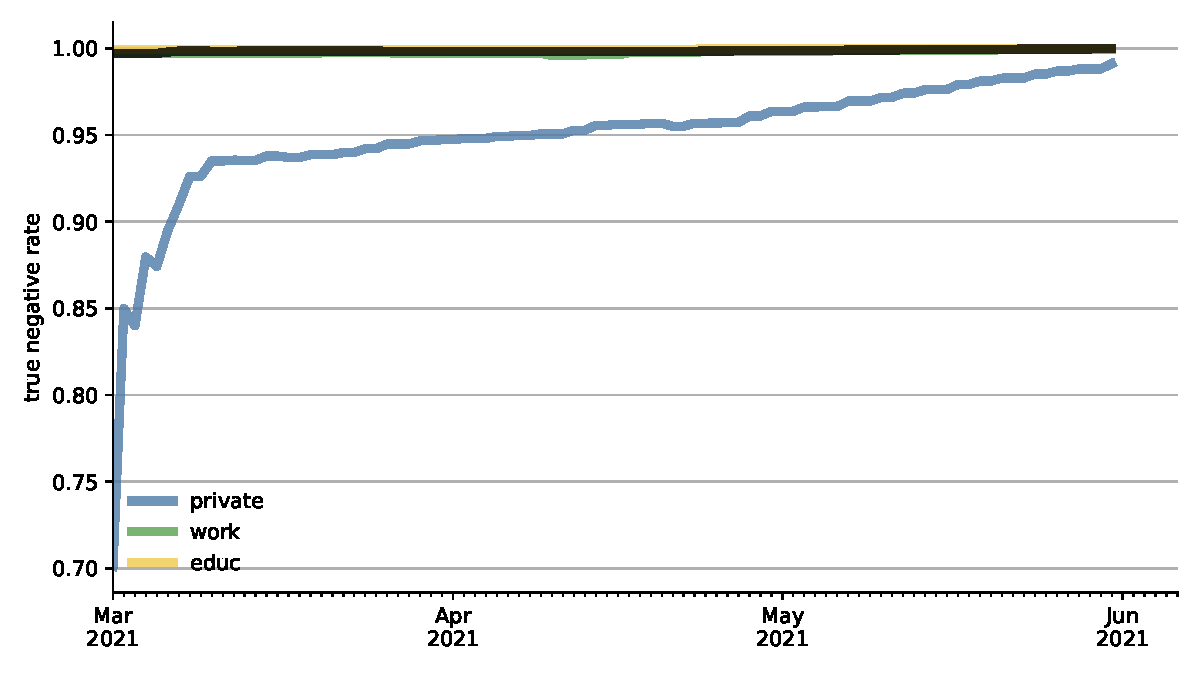
\includegraphics[width=\textwidth]{figures/results/figures/rapid_test_statistics/true_negative_rate}
    %     \caption{Rate of True Negative Rapid Tests by Channel}
    %     \label{fig:rapid_tests_true_negative_rate}
    % \end{subfigure}
    \hfill
    \begin{subfigure}[b]{0.425\textwidth}
        \centering
        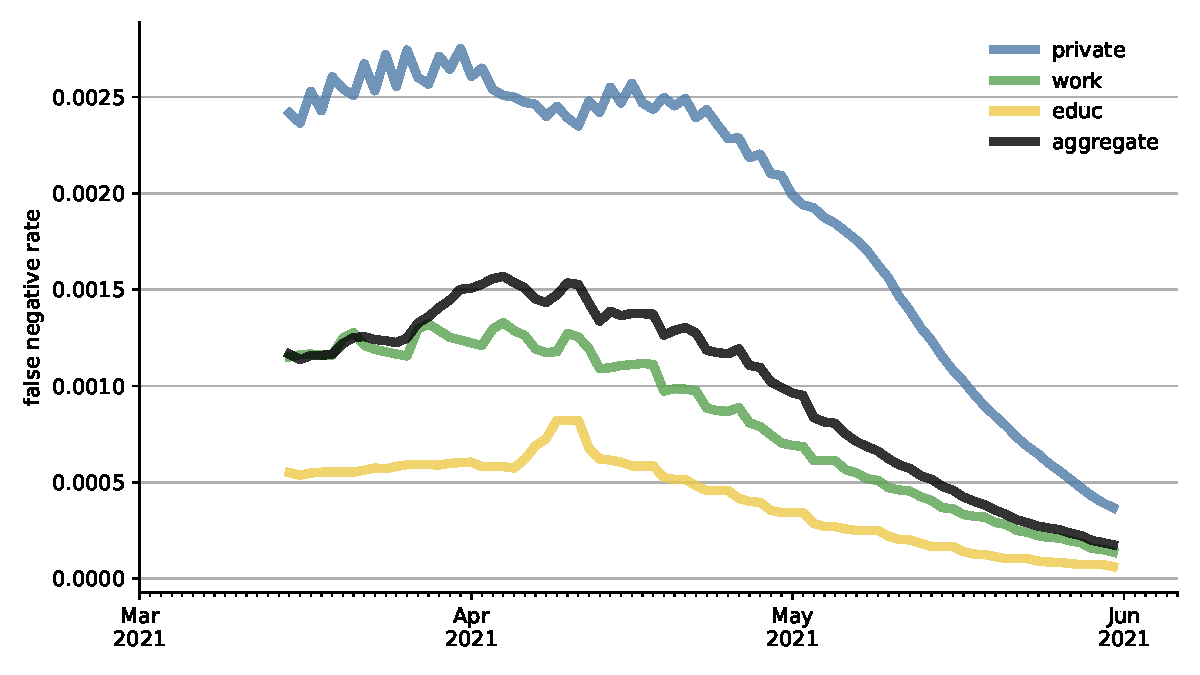
\includegraphics[width=\textwidth]{figures/results/figures/rapid_test_statistics/false_negative_rate}
        \caption{Rate of False Negative Rapid Tests by Channel}
        \label{fig:rapid_tests_false_negative_rate}
    \end{subfigure}
    \vskip3ex
    \caption{Rapid Test Rates by Channel}
    \label{fig:rapid_test_results_rates}

    \floatfoot{\noindent \textit{Note:}
        The left panel shows the share of positive tests that are given to people who are not
        infected. This share is large as can be expected with a very low baseline rate of
        positive individuals. As the incidence in the population drops, the false positive
        rate increases. An exception are the private rapid tests because they are --
        especially when the incidence is high -- often triggered by events that make it
        likely that the test taker is infected and therefore their false positive rate is
        much lower. The right panel shows the false negative rate in the population, i.e. the
        share of negative test results that are mistakenly given to infected individuals.
        This is very low because there are many truly negative tests in times of low
        incidences and large scale screening tests.}
\end{figure}

\FloatBarrier

